\documentclass[ucs,9pt]{beamer}
\setbeamertemplate{navigation symbols}{}
% remove this line and the "ucs" option to the documentclass when your editor is not utf8-capable
\usepackage[utf8x]{inputenc}    % to make utf-8 input possible
\usepackage[english]{babel}     % hyphenation etc., alternatively use 'german' as parameter
%\usepackage{listings}

% Template for talks using the Corporate Design of the Freie Universitaet
%   Berlin, created following the guidelines on www.fu-berlin.de/cd by
%   Tobias G. Pfeiffer, <tobias.pfeiffer@math.fu-berlin.de>
% This file can be redistributed and/or modified in any way you like.
%   If you feel you have done significant improvements to this template,
%   please consider providing your modified version to
%   https://www.mi.fu-berlin.de/w/Mi/BeamerTemplateCorporateDesign

\usepackage{amsmath,dsfont,listings}

%%% FU logo
% small version for upper right corner of normal pages
\pgfdeclareimage[height=0.9cm]{university-logo}{FULogo_RGB}
\logo{\pgfuseimage{university-logo}}
% large version for upper right corner of title page
\pgfdeclareimage[height=1.085cm]{big-university-logo}{FULogo_RGB}
\newcommand{\titleimage}[1]{\pgfdeclareimage[height=2.92cm]{title-image}{#1}}
\titlegraphic{\pgfuseimage{title-image}}
%%% end FU logo

% NOTE: 1cm = 0.393 in = 28.346 pt;    1 pt = 1/72 in = 0.0352 cm
\setbeamersize{text margin right=3.5mm, text margin left=7.5mm}  % text margin

% colors to be used
\definecolor{text-grey}{rgb}{0.45, 0.45, 0.45} % grey text on white background
\definecolor{bg-grey}{rgb}{0.66, 0.65, 0.60} % grey background (for white text)
\definecolor{fu-blue}{RGB}{0, 51, 102} % blue text
\definecolor{fu-green}{RGB}{153, 204, 0} % green text
\definecolor{fu-red}{RGB}{204, 0, 0} % red text (used by \alert)

% switch off the sidebars
% TODO: loading \useoutertheme{sidebar} (which is maybe wanted) also inserts
%   a sidebar on title page (unwanted), also indents the page title (unwanted?),
%   and duplicates the navigation symbols (unwanted)
\setbeamersize{sidebar width left=0cm, sidebar width right=0mm}
\setbeamertemplate{sidebar right}{}
\setbeamertemplate{sidebar left}{}
%    XOR
% \useoutertheme{sidebar}

% frame title
% is truncated before logo and splits on two lines
% if neccessary (or manually using \\)
\setbeamertemplate{frametitle}{%
    \vskip-30pt \color{text-grey}\large%
    \begin{minipage}[b][23pt]{80.5mm}%
    \flushleft\insertframetitle%
    \end{minipage}%
}

%%% title page
% TODO: get rid of the navigation symbols on the title page.
%   actually, \frame[plain] *should* remove them...
\setbeamertemplate{title page}{
% upper right: FU logo
\vskip2pt\hfill\pgfuseimage{big-university-logo} \\
\vskip6pt\hskip3pt
% title image of the presentation
\begin{minipage}{11.6cm}
\hspace{-1mm}\inserttitlegraphic
\end{minipage}

% set the title and the author
\vskip14pt
\parbox[top][1.35cm][c]{11cm}{\color{text-grey}\inserttitle \\ \small \insertsubtitle}
\vskip11pt
\parbox[top][1.35cm][c]{11cm}{\small \insertauthor \\ \insertinstitute \\[3mm] \insertdate}
}
%%% end title page

%%% colors
\usecolortheme{lily}
\setbeamercolor*{normal text}{fg=black,bg=white}
\setbeamercolor*{alerted text}{fg=fu-red}
\setbeamercolor*{example text}{fg=fu-green}
\setbeamercolor*{structure}{fg=fu-blue}

\setbeamercolor*{block title}{fg=white,bg=black!50}
\setbeamercolor*{block title alerted}{fg=white,bg=black!50}
\setbeamercolor*{block title example}{fg=white,bg=black!50}

\setbeamercolor*{block body}{bg=black!10}
\setbeamercolor*{block body alerted}{bg=black!10}
\setbeamercolor*{block body example}{bg=black!10}

\setbeamercolor{bibliography entry author}{fg=fu-blue}
% TODO: this doesn't work at all:
\setbeamercolor{bibliography entry journal}{fg=text-grey}

\setbeamercolor{item}{fg=fu-blue}
\setbeamercolor{navigation symbols}{fg=text-grey,bg=bg-grey}
%%% end colors

%%% headline
\setbeamertemplate{headline}{
\vskip4pt\hfill\insertlogo\hspace{3.5mm} % logo on the right

\vskip6pt\color{fu-blue}\rule{\textwidth}{0.4pt} % horizontal line
}
%%% end headline

%%% footline
\newcommand{\footlinetext}{\insertshortinstitute, \insertshorttitle, \insertshortdate}
\setbeamertemplate{footline}{
\vskip5pt\color{fu-blue}\rule{\textwidth}{0.4pt}\\ % horizontal line
\vskip2pt
\makebox[123mm]{\hspace{7.5mm}
\color{fu-blue}\footlinetext
\hfill \raisebox{-1pt}{\usebeamertemplate***{navigation symbols}}
\hfill \insertframenumber}
\vskip4pt
}
%%% end footline

%%% settings for listings package
\lstset{extendedchars=true, showstringspaces=false, basicstyle=\footnotesize\sffamily, tabsize=2, breaklines=true, breakindent=10pt, frame=l, columns=fullflexible}
\lstset{language=Java} % this sets the syntax highlighting
\lstset{mathescape=true} % this switches on $...$ substitution in code
% enables UTF-8 in source code:
\lstset{literate={ä}{{\"a}}1 {ö}{{\"o}}1 {ü}{{\"u}}1 {Ä}{{\"A}}1 {Ö}{{\"O}}1 {Ü}{{\"U}}1 {ß}{\ss}1}
%%% end listings  % THIS is the line that includes the FU template!

\usepackage{arev,t1enc} % looks nicer than the standard sans-serif font
% if you experience problems, comment out the line above and change
% the documentclass option "9pt" to "10pt"

% image to be shown on the title page (without file extension, should be pdf or png)
\titleimage{mi-bildbalken}
\title[Para Sort] % (optional, use only with long paper titles)
{Parallele Sortierung}

%\subtitle
%{Include Only If Paper Has a Subtitle}

\author[] % (optional, use only with lots of authors)
{Björn Rathjen \and Patrick Winterstein}
% - Give the names in the same order as the appear in the paper.

\institute[FU Berlin] % (optional, but mostly needed)
{Freie Universität Berlin}

\date[ProSem Algo]
{Proseminar Algorithmen, SS14}

%\subject{Theoretical Computer Science}
% This is only inserted into the PDF information catalog. Can be left
% out.

% you can redefine the text shown in the footline. use a combination of
% \insertshortauthor, \insertshortinstitute, \insertshorttitle, \insertshortdate, ...
\renewcommand{\footlinetext}{\insertshortinstitute, \insertshorttitle, \insertshortdate}

\AtBeginSection[]
{
	\begin{frame}<beamer>
		\tableofcontents[currentsection,hideothersubsubsections,hideothersubsections]
	\end{frame}
}

\begin{document}

%Titelblatt
\begin{frame}[plain]
  \titlepage
\end{frame}
 
%Inhaltsverzeichnis
\begin{frame}{Inhalt}
  \tableofcontents[hideallsubsubsections,allowframebreaks] %currentsection,hideallsubsections,hideallsubsubsections
  % You might wish to add the option [pausesections]
\end{frame}

% Motivation
\section{Motivation}
    
\begin{frame}{Motivation : Allgemein}
    ist Basis für :
    \begin{itemize}
        \item Suche
        \item (Sortierung)
        \begin{itemize}
            \item Listen
            \item Wörterbücher
            \item ... 
        \end{itemize}
        \item Ist dies auch in Hardware möglich ?
    \end{itemize}
\end{frame}

\section{Grundlage des Sortierens}
\subsection{Komparator}
\begin{frame}{Aufbau}
    \begin{minipage}[c]{14.5cm}
    		\begin{minipage}[c]{5cm}
        		\begin{itemize}
            		\item 2 Eingänge
	            	\item vergleichender Baustein
    		        	\item 2 Ausgänge
        		\end{itemize}
	    \end{minipage}
%    		\hfill
		\begin{minipage}[c]{5cm}
			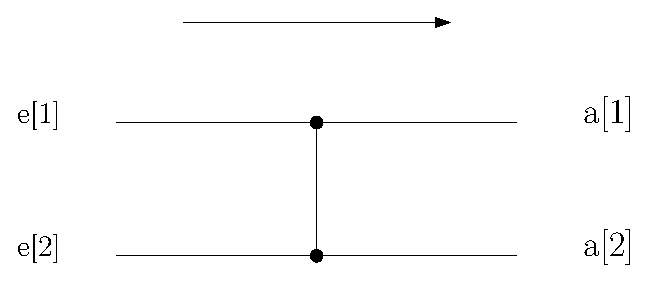
\includegraphics[scale=0.5]{Komparator1.eps}
	 	\end{minipage}
    \end{minipage}
\end{frame}

%Pseudocode
\begin{frame}[fragile]{Vergleichender Baustein (ii)}
\begin{lstlisting}[laguage={inform},tabsize=4]
    void comp(chan in1, in2, out1 out2){
        a = <- in1;
        b = <- in2;
        
        if (a < b){
            out1 <- a;
            out2 <- b;
            return void;
        }
        out1 <- b;
        out2	 <- a;
        return void;
    }
\end{lstlisting}
\end{frame}

\section{Sortiernetzwerk}
\subsection{Aufbau}

\begin{frame}{Erweiterung : Aufbau}
    \begin{itemize}
        \item mehrere Eingabeleitungen
        \item Vergleichende Schritte müssen dazwischen laufen
        \item mehrere Ausgabeleitungen sortierte Ausgabe
    \end{itemize}
\end{frame}

\subsubsection*{nativer Ansatz}
\begin{frame}{nativ : Aufgabe}
\begin{semiverbatim}
    \uncover<1-> {Aufgabe
        \begin{itemize}
            \item Resultat soll sortierte Eingabe sein
            \end{itemize}}
    \uncover<2-> {\item grundlegendes Prinzip
        \begin{itemize}
            \item intuitiver Einsatz von Vergleichen
            \item Schrittweises sortieren
        \end{itemize}}
\end{semiverbatim}
\end{frame}

\begin{frame}{nativ : grundlegendes Prinzip}
\begin{center}
    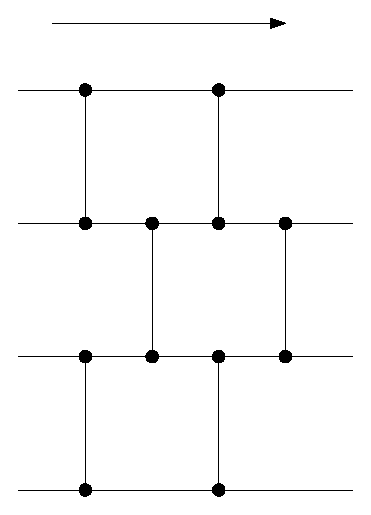
\includegraphics[scale=0.8]{bild2Komparatornetzwerk.eps}
\end{center}
\end{frame}

\begin{frame}{Demonstration}
\begin{center}
   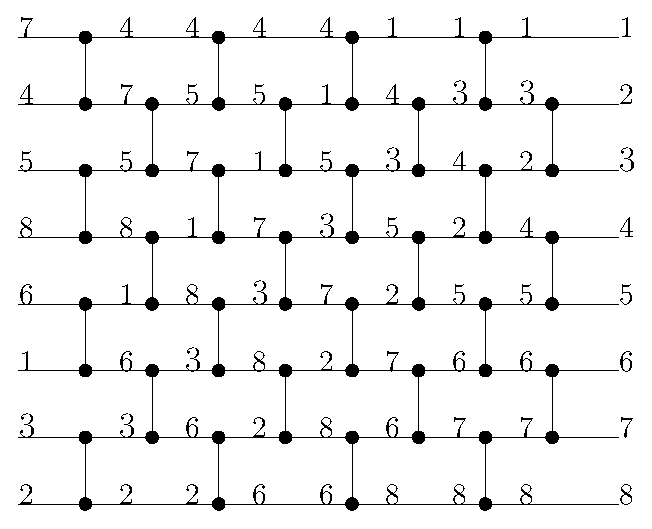
\includegraphics[scale=0.8]{bild2beispiel.eps}
  \end{center}
\end{frame}

\subsection{Korrektheit}
\begin{frame}{0,1-Prinzip}
\begin{theorem} 
Wenn es eine Folge A gibt, die ein Sortiernetzwerk nicht sortiert, so existiert auch eine 0,1-Folge, die von diesem Netzwerk nicht sortiert wird.
\end{theorem}
\begin{proof}
{\color{red} fill}
\end{proof}
\end{frame}

\begin{frame}{Ansatz}
    man kann jede Zahlenfolge durch eine 0,1 Folge repräsentieren
    $$
    f(c) = \begin{cases} 0 , & if \;\;c < k \\
    1 , & if \;\;c \geq k
    \end{cases}$$
\end{frame}

\begin{frame}{0,1- Beispiel}
\begin{semiverbatim}
\uncover<1-> {
\begin{center}
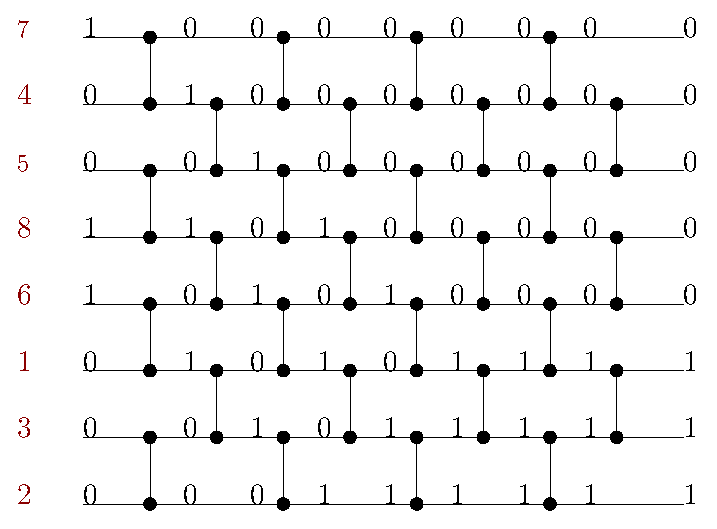
\includegraphics[scale=0.8]{01beispiel.eps}
\end{center}
}
\uncover<2-> {\begin{center} {\color{green}Beispiel an der Tafel ?}\end{center} }
\end{semiverbatim}
\end{frame}

\subsection*{Aufbau eines effektieveren Netzwerks}
%Einsatzorte
\begin{frame}{effektiveres Netzwerk}
    \begin{semiverbatim}[fontfamily=ucs]
    		\uncover<1-> { }
        \uncover<2-> {Aufgabe :
            \begin{itemize}
                \item Resultat soll sortierte Eingabe sein
                \item \alert{soll effizient sein}
            \end{itemize}}
        \uncover<3-> {grundlegendes Prinzip :
            \begin{itemize}
                \item intuitiver Einsatz von Vergleichen
                \item[]\alert{+ Einbezug von Teile und Herrscher}
                % mh sehr leere Folien
            \end{itemize}}
    \end{semiverbatim}
\end{frame}

\begin{frame}{Aufteilung}
\begin{center}
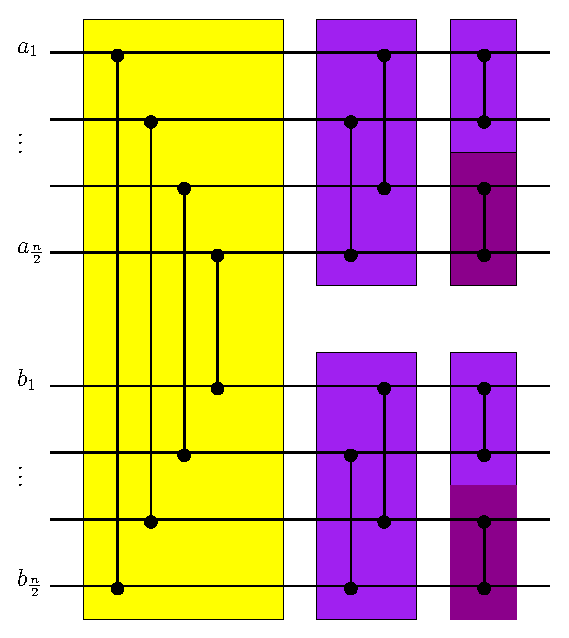
\includegraphics[scale=0.6]{bitonmischer.eps}
\end{center}
\end{frame}

\begin{frame}{Biton -Sortierer : Aufbau}
    \begin{center}
    		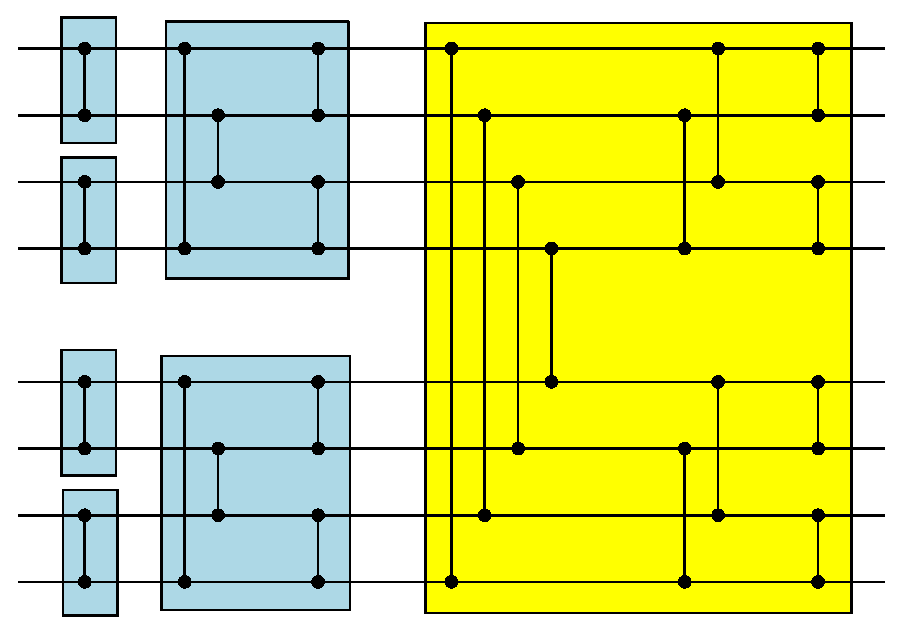
\includegraphics[scale=0.6]{biton2.eps}
    \end{center}
\end{frame}

\begin{frame}{Demonstration}
    Bild kleiner Zahlenfolge 4-8-16\\
    Beispiel
\end{frame}

\section{Laufzeit}
\subsection{Herleitung}
\begin{frame}
\uncover<2-> {$$ 1 $$}
\uncover<3-> {$$ 1 + 2 $$ }
\uncover<4-> {$$ 1 + 2 + … + k-1 + k  = \sum_{i=1}^k i$$ }
\uncover<5-> {$$ \frac{k \cdot (k+1)}{2} | n = 2^k $$}
\uncover<1-> {$$ \frac{1}{2}\; \cdot\;\log_2 n \;\; (\log_2 n\;+\;1)$$}
\end{frame}

\subsection{Vergleich mit Software sortieren}
\begin{frame}
	\begin{itemize}
		\item Unterschiedliche Betrachtungen Schritte gegen Vergleiche, Versuch der Darstellung
	 	\item Abhängigkeit von der Eingabe
	 	\item Bezug zum vorherigen Vergleich
	\end{itemize}
\end{frame}

\begin{frame}{Bubblesort im Hardwarenetz}
	\begin{center}
	    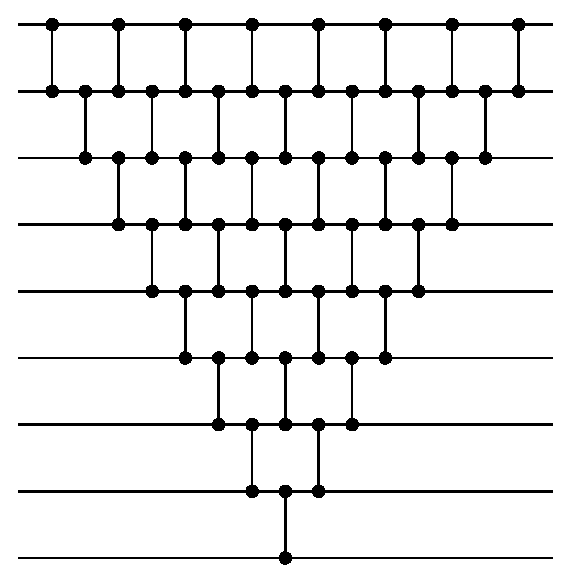
\includegraphics[scale=0.65]{bubblesort.eps}
	\end{center}
\end{frame}

\begin{frame}{Softwaresortieren im Hardwarenetz}
    \begin{center}
    		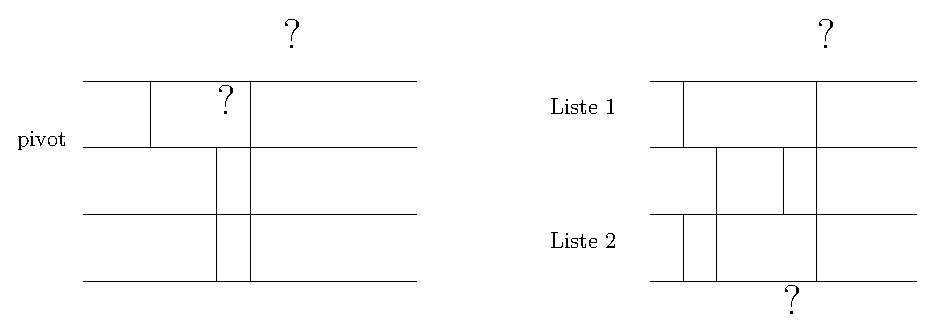
\includegraphics[scale=0.65]{mergesort.eps}
\end{center}     
 wo ist das Pivot Element ?\\
        Wo ist nun das größte Element ?
\end{frame}

\section{Gegenüberstellung}
\begin{frame}
    \begin{itemize}
        \item Geschwindigkeit vs Variabilität
        \begin{itemize}
            \item hohe Geschwindigkeit durch direkte Hardware Implementriegung
            \item starre Struktur , bildet Rahmen der Möglichkeiten
            \item stark typisierte Eingabe
        \end{itemize}
    \item Hardwareaufwand vs Softwareaufwand
        \begin{itemize}
            \item Software zur Auswertung keine zum sortieren
            \item geringe Skalierbarkeit
            \item hoher Aufwand wenn Eingabelimit überschritten wird
            \item nur lokal
            \item Hardware Konzeption eventuell aufwendiger
        \end{itemize}
    \end{itemize}
\end{frame}

\section{Zusammenfassung}
\begin{frame}{Zusammenfassung}
\begin{itemize}
  \item paralleles sortieren ist schnell und effizient 
  \item problemabhängige Lösung
  \item starr, nicht universell
\end{itemize}
\end{frame}

\section{Ausblick}
\begin{frame}{Ausblick}
weiter
\end{frame}

\subsection{Hybercube}
\begin{frame}{Hyprecube}
?¿
\end{frame}

\begin{frame}{Aufbau}
structur
\end{frame}

\begin{frame}{Funktion}

\end{frame}

%Ende
\begin{frame}{Ende}
    Fragen, Anregungen?\\
    (keine Liederwünsche)
\end{frame}

\subsection{Anhang}
\appendix

\section<presentation>*{\appendixname}
\subsection<presentation>*{For Further Reading}

\begin{frame}[allowframebreaks]
  \frametitle<presentation>{For Further Reading}
    
  \begin{thebibliography}{10}
    
  \beamertemplatebookbibitems
  % Start with overview books.

  \bibitem{}
    A.~Author.
    \newblock {\em Taschenbuch der Algorithmen}.
    \newblock Springer Verlag , 2008.
    
  \bibitem{Author1990}
    Tom Leighton.
    \newblock {\em Einführung in Parallele Algorithmen und Architekturen}{\\Gitter, Bäume und Hypercubes}.
    \newblock Thomsom Publisching , 1997.
 
    
  \beamertemplatearticlebibitems
  % Followed by interesting articles. Keep the list short. 

  \bibitem{0,1-Prinzip}
    S.~Someone.
   % \href{http://www.iti.fh-flensburg.de/lang/algorithmen/sortieren/networks/nulleins.htm}
    \newblock 
    \newblock {http://www.iti.fh-flensburg.de/lang/algorithmen/sortieren/networks/nulleins.htm}
    
  \end{thebibliography}
\end{frame}

\end{document}

\begin{frame}{Make Titles Informative. Use Uppercase Letters. Long Titles are Split Automatically.}{Subtitles are optional.}
  % - A title should summarize the slide in an understandable fashion
  %   for anyone how does not follow everything on the slide itself.
  \begin{itemize}
  \item
    Use \texttt{itemize} a lot.
  \item
   	Kurze Sätze benutzen.
  \end{itemize}
\end{frame}

\begin{frame}{Make Titles Informative.}

  You can create overlays\dots
  \begin{itemize}
  \item using the \texttt{pause} command:
    \begin{itemize}
    \item
      First item.
      \pause
    \item    
      Second item.
    \end{itemize}
  \item
    using overlay specifications:
    \begin{itemize}
    \item<3->
      First item.
    \item<4->
      Second item.
    \end{itemize}
  \item
    using the general \texttt{uncover} command:
    \begin{itemize}
      \uncover<5->{\item
        First item.}
      \uncover<6->{\item
        Second item.}
    \end{itemize}
  \end{itemize}
\end{frame}

\begin{frame}[fragile]{An old algorithm}
% NB. listings is quite powerful, but not well suited to be used with beamer
%  consider using semiverbatim or the like, see below
\begin{lstlisting}[language=C]
int main (void)
{
  std::vector<bool> is_prime (100, true);
  for (int i = 2; i < 100; i++)
    if (is_prime[i])
      {
        std::cout << i << " ";
        for (int j = i; j < 100;
            is_prime [j] = false, j+=i);
      }
  return 0;
}
\end{lstlisting}
\end{frame}

\begin{frame}[fragile]
  \frametitle{An Algorithm For Finding Primes Numbers.}
\begin{semiverbatim}
\uncover<1->{\alert<0>{int main (void)}}
\uncover<1->{\alert<0>{\{}}
\uncover<1->{\alert<1>{ \alert<4>{std::}vector<bool> is_prime (100, true);}}
\uncover<1->{\alert<1>{ for (int i = 2; i < 100; i++)}}
\uncover<2->{\alert<2>{    if (is_prime[i])}}
\uncover<2->{\alert<0>{      \{}}
\uncover<3->{\alert<3>{        \alert<4>{std::}cout << i << " ";}}
\uncover<3->{\alert<3>{        for (int j = i; j < 100;}}
\uncover<3->{\alert<3>{             is_prime [j] = false, j+=i);}}
\uncover<2->{\alert<0>{      \}}}
\uncover<1->{\alert<0>{ return 0;}}
\uncover<1->{\alert<0>{\}}}
\end{semiverbatim}
  \visible<4->{Note the use of \alert{\texttt{std::}}.}
\end{frame}



\begin{frame}{Make Titles Informative.}
  \begin{example}
    \begin{itemize}
    \item 2 is prime (two divisors: 1 and 2).
    \item 3 is prime (two divisors: 1 and 3).
    \item 4 is not prime (\alert{three} divisors: 1, 2, and 4).
    \end{itemize}
  \end{example}
\end{frame}

\begin{frame}{Make Titles Informative.}
\begin{theorem}
 There is no largest prime number and, in addition, $$\int_\Omega \nabla u \cdot \nabla v = - \int_\Omega u \Delta v + \int_{\partial\Omega} u v n$$
 \end{theorem}
 \begin{proof}
 \begin{enumerate}
 \item<1-> Suppose $p$ were the largest prime number.
 \item<2-> Let $q$ be the product of the first $p$ numbers.
 \item<3-> Then $q + 1$ is not divisible by any of them.
 \item<1-> Thus $q + 1$ is also prime and greater than $p$.\qedhere
 \end{enumerate} 
 \end{proof}
 \uncover<4->{The proof used \textit{reductio ad absurdum}.}
\end{frame}

\begin{frame}{Make Titles Informative.}
\end{frame}



\begin{frame}{Summary}

  % Keep the summary *very short*.
  \begin{itemize}
  \item
    The \alert{first main message} of your talk in one or two lines.
  \item
    The \alert{second main message} of your talk in one or two lines.
  \item
    Perhaps a \alert{third message}, but not more than that.
  \end{itemize}
  
  % The following outlook is optional.
  \vskip0pt plus.5fill
  \begin{itemize}
  \item
    Outlook
    \begin{itemize}
    \item
      Something you haven't solved.
    \item
      Something else you haven't solved.
    \end{itemize}
  \end{itemize}
\end{frame}
